\graphicspath{{chapters/IGVimages/}}

\chapter*{IGV (Integrative Genomics Viewer)}

\section*{Main characteristics}
The human genome nowadays is being explored extensively thanks to of exons and
whole-genome sequencing, epigenetic surveys, expression profiling of coding and
noncoding RNAs, single nucleotide polymorphism (SNP) and copy number profiling,
and functional assays. Those findings are essential to pave the way for the
future \textbf{precision medicine}. This is an approach for desease treatment and
prevention that takes into account individual variability in genes, environment,
and lifestyle for each person. The right drug, at the right time and at the
right dose for each individual. 

\begin{figure}[H]
    \caption{All the important usages of IGV}
    \centering
    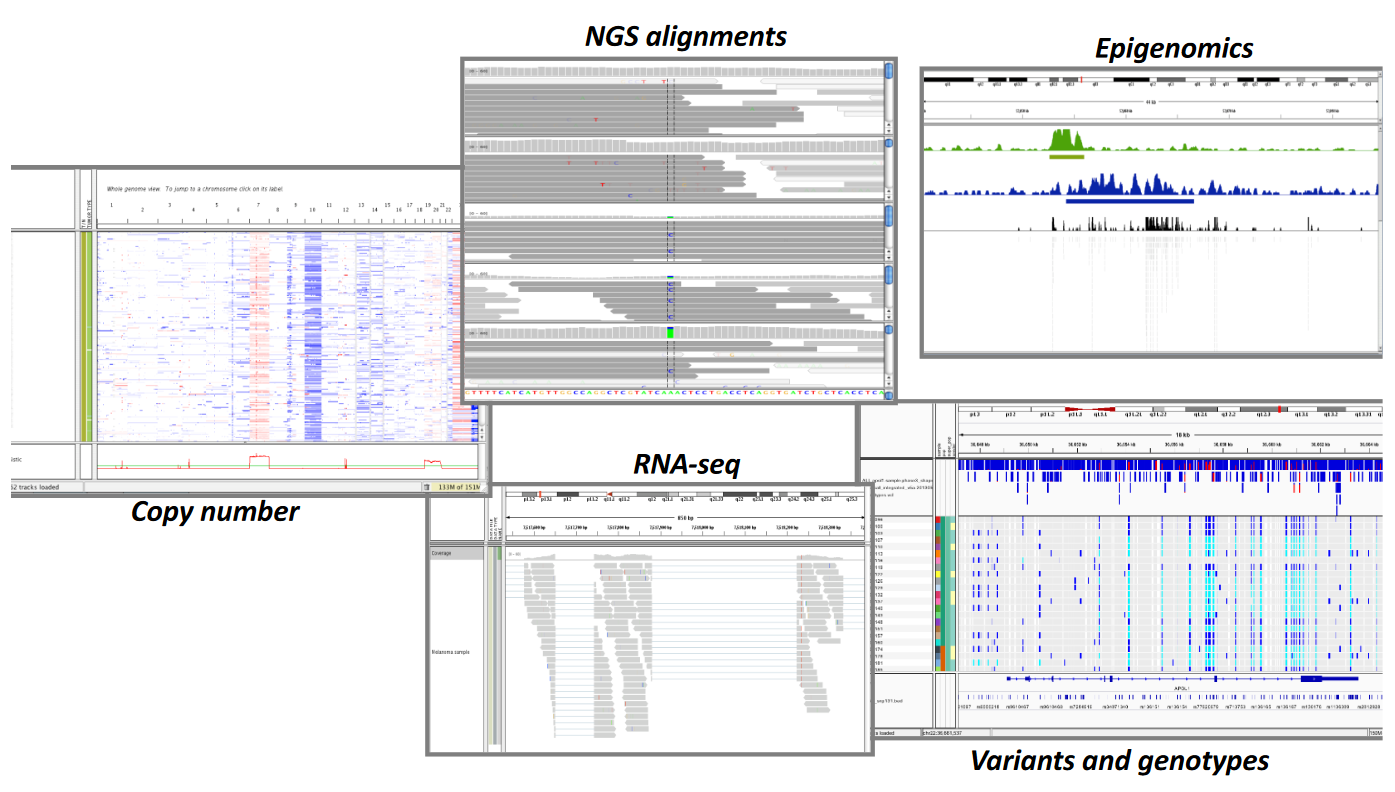
\includegraphics[width=0.6\textwidth]{usagesIGV.PNG}
    \label{IGVusages}
\end{figure}

The IGV software is an \textbf{high-performance lightweight visualization tool}
for interactive exploration of large, integrated genomic datasets. It supports a
\underline{wide variety of data types}, including next-generation sequence data,
and genomic annotations. Data sets can be loaded from local or remote sources,
including cloud-based resources. \\
It allows to move, zoom in and out quickly over different genomic scales, and also to
jump in precise positions of the sequence. It is possible to search for genomic coordinates or gene names. Pixel
resolution errors, occuring when data density exceeds the constraint given by
the number of pixels available for display, could be solved through data
aggregation. As the user zooms below the ~50 kb range, individual aligned reads
become visible. It is possible then to zoom further, and see the bases at each
position.
 
Annotations for specific genomes could be found consulting the UCSC Table Browser \href{http://genome.ucsc.edu/cgi-bin/hgTables}{(UCSC table)}.

Other information are present in the
\href{https://authors.library.caltech.edu/72234/2/nbt.1754-S1.pdf}{Supplementaty
information - Integrative Genomics Viewer} pdf file.

%#TODO For each resolution scale (“zoom level”), the aggregated data is divided into
%tiles that correspond to a region viewable on a typical user display. Each tile
%is subdivided into bins, with the width of a bin chosen to correspond to the
%width represented by a pixel at that resolution scale. During the
%pre-computation step, data in each bin is aggregated into one or more summary
%statistics as specified by the user. Data Format: the corresponding data tiles
%for each zoom level are stored in the binary Tiled Data Format, or TDF, which
%has been optimized for fast tile retrieval. - tile sizes for each zoom level
%are constant and small, - only the data needed to render the view at the
%resolution supported by the screen display. - a single tile at the lowest
%resolution (spanning the entire genome) has the same memory footprint as a tile
%at the very high zoom levels (might span only a few kilobases). Tiles no longer
%in view are discarded as needed to free memory. Navigation through a data set
%is similar to that of Google Maps, allowing the user to zoom and pan seamlessly
%across the genome at any level of detail from whole genome to base pair.

\begin{figure}[H]
    \caption{All the important elements to navigate into IGV are reported in the figure}
    \centering
    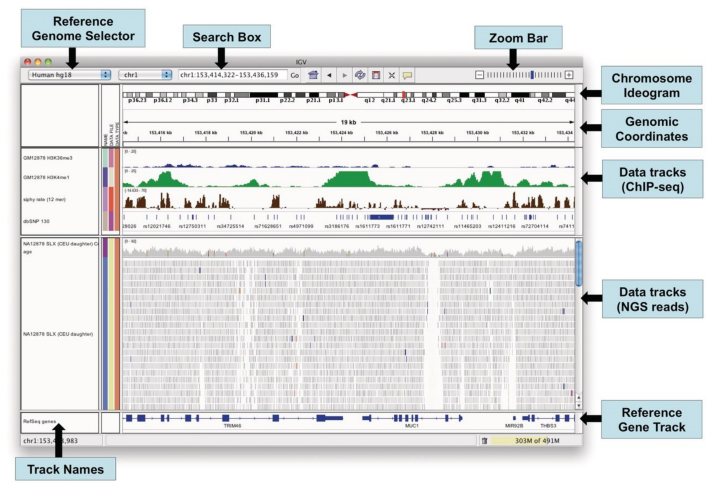
\includegraphics[width=0.7\textwidth]{IGVview.PNG}
    \label{IGVnavigation}
\end{figure}
\begin{figure}[H]
    \caption{}
    \centering
    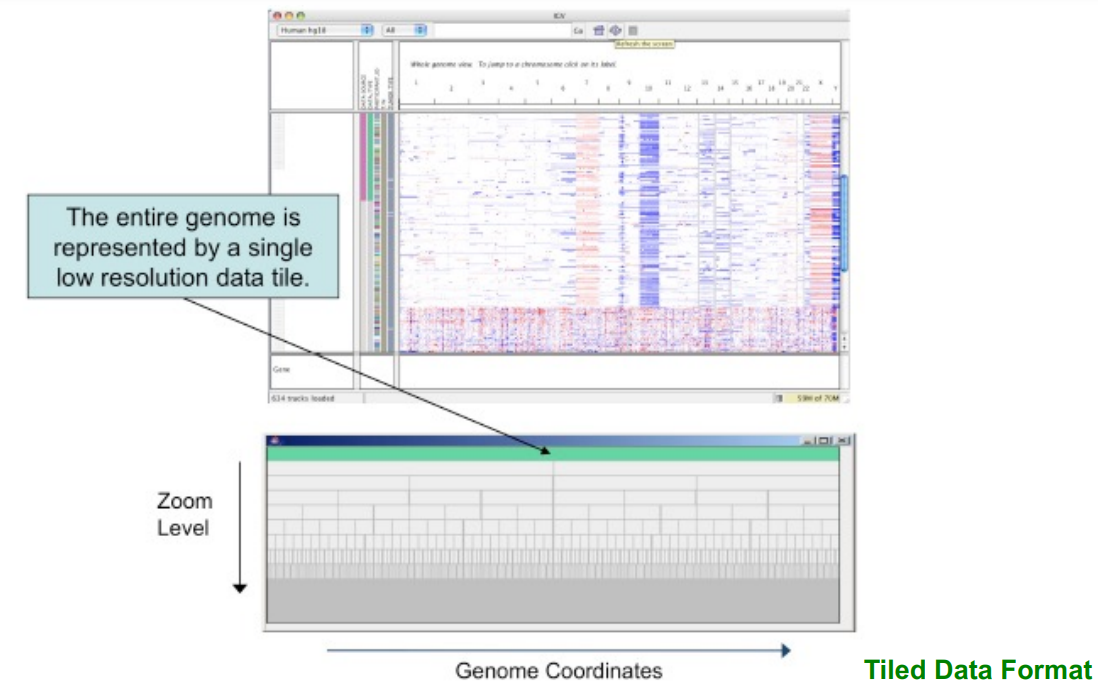
\includegraphics[width=0.6\textwidth]{Tiles.PNG}
    \label{Til}
\end{figure}
\begin{figure}[H]
    \caption{}
    \centering
    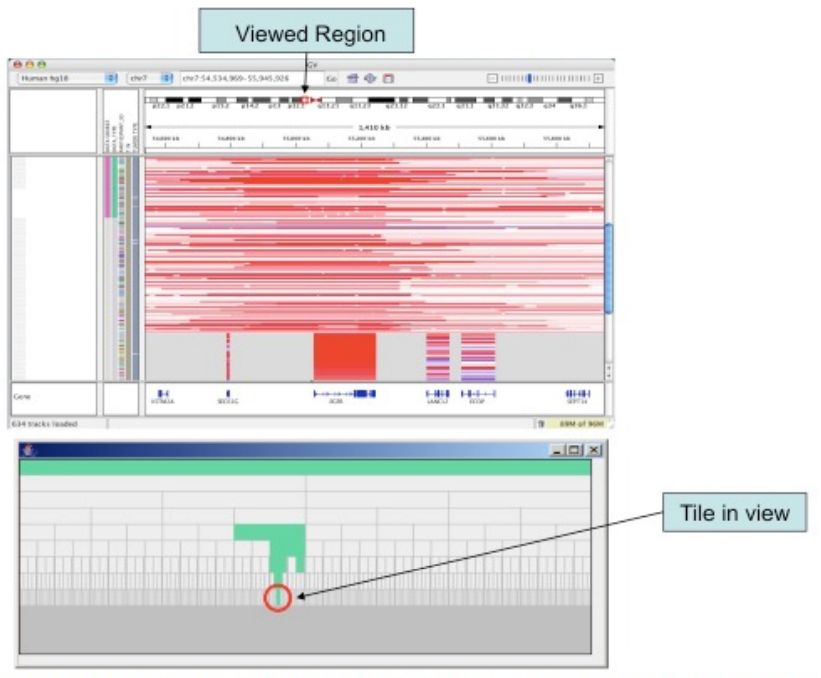
\includegraphics[width=0.6\textwidth]{TileView.PNG}
    \label{img: TileV}
\end{figure}
\begin{figure}[H]
    \caption{}
    \centering
    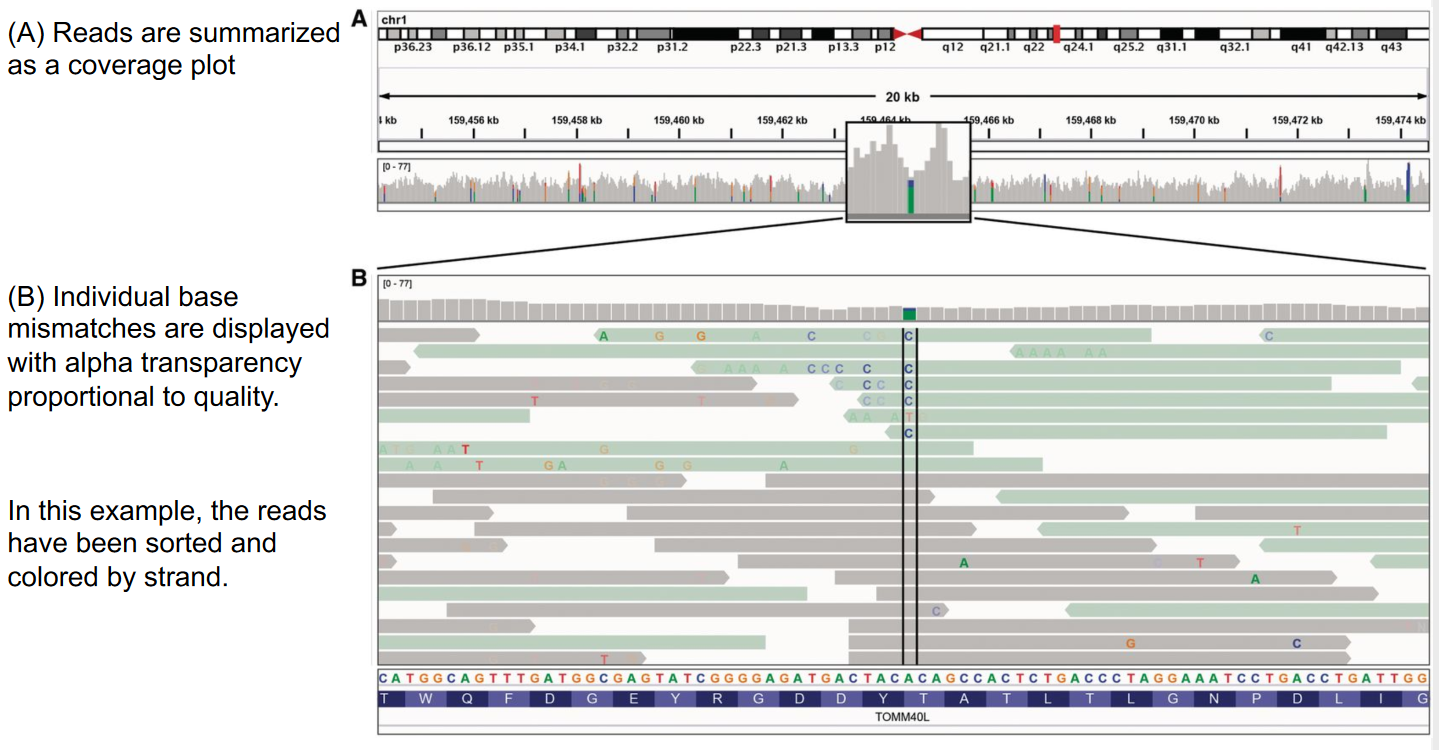
\includegraphics[width=0.6\textwidth]{IGVReadsView.PNG}
    \label{ViewReads}
\end{figure} 


\subsection*{igvtools}
Igvtools comprises a set of utilities for preparing large files for efficient display.

\begin{figure}[H]
    \caption{igvtools possible operations, the "count" function allows to generate coverage data, and it takes in input a BAM file. The obtained data could be then loaded with the "Load pre-computed coverage data" commandq}
    \centering
    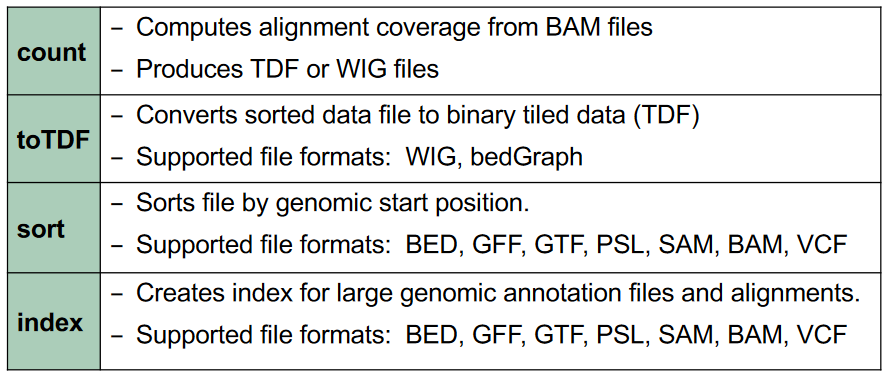
\includegraphics[width=0.6\textwidth]{igvtools.PNG}
\end{figure}

\subsection*{Session Files}
Sessions are an integral part of IGV, allowing users to share their data and
views with other users simply and accurately. Session files describe the session
in XML.

\begin{figure}[H]
    \caption{Structure of the XML file}
    \centering
    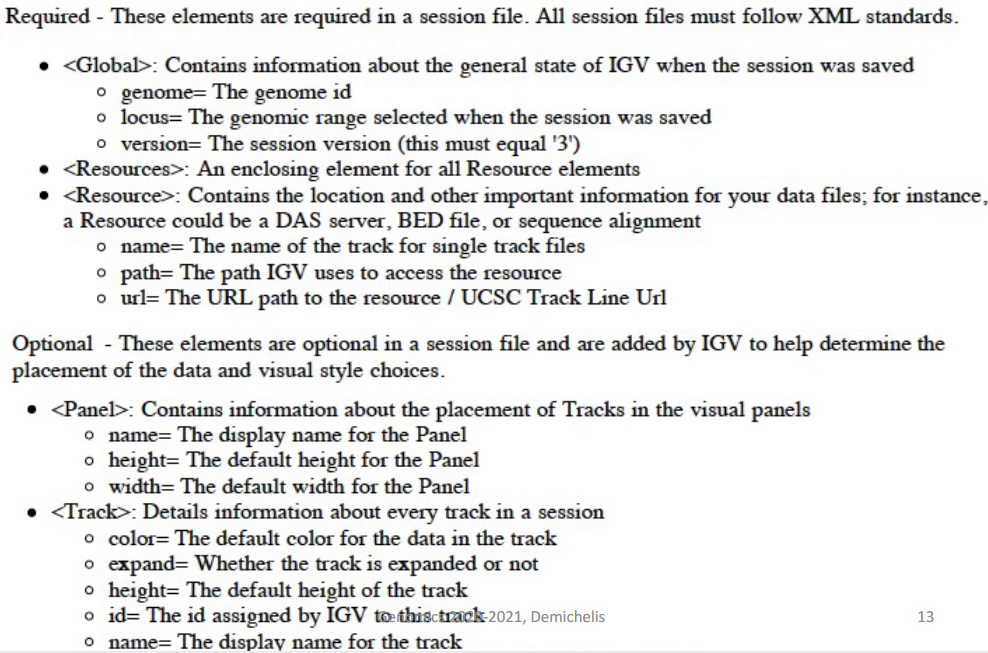
\includegraphics[width=0.75\textwidth]{structureXMLfile.PNG}
    \label{XMLfile}
\end{figure} 



\section*{Some of the main utilizations}
\textit{(I will not write down all the passages needed to obtain the figures represented
below, as they are included in the exercise file delivered by the professor)}

\subsection*{RNA-seq alignments}

\begin{figure}[H]
    \caption{the height depends on the quantity of reads connecting the different exons.}
    \centering
    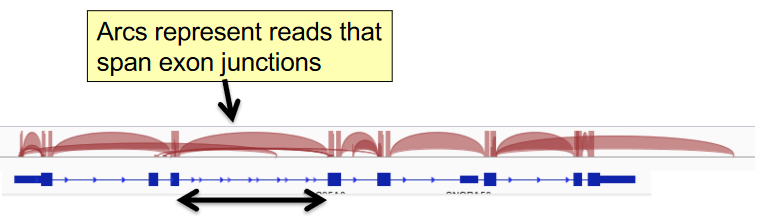
\includegraphics[width=0.6\textwidth]{RNAseqAlign.PNG}
\end{figure}

\begin{figure}[H]
    \caption{\textbf{Sashami plots}: The number of reads connecting exosomes are
    represented here on the curved lines. The peaks represent coverage within
    exons.}
    \centering
    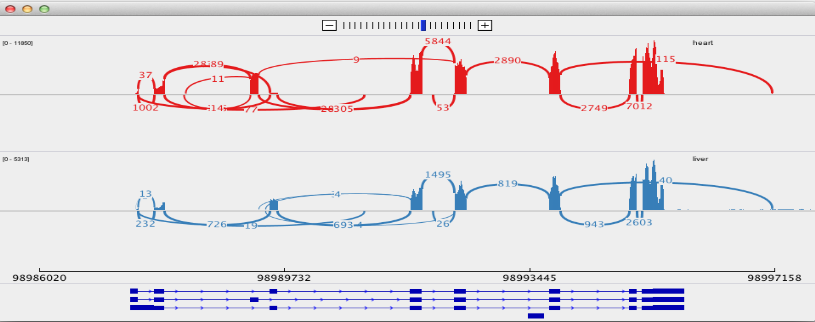
\includegraphics[width=0.6\textwidth]{sashamiplot.PNG}
\end{figure}

\subsection*{Study of variants}
It is possible to study variants from different samples.

\begin{figure}[H]
    \centering
    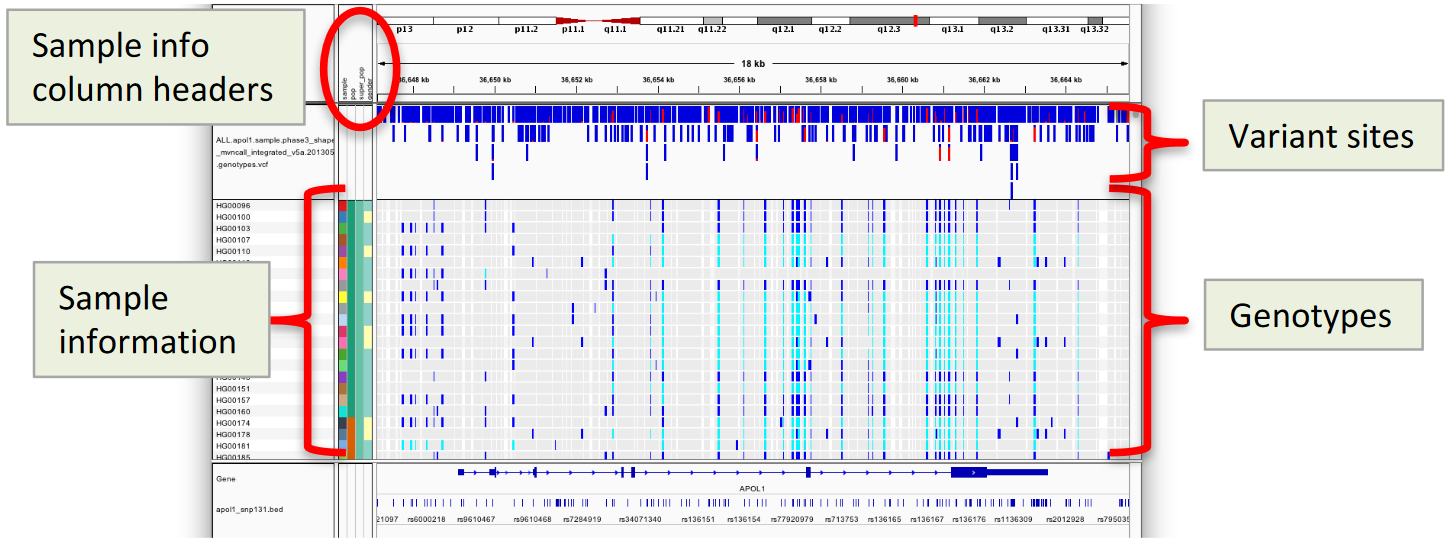
\includegraphics[width=0.6\textwidth]{variantsView.PNG}
\end{figure}

It is also possible to sort the samples in different ways and to group them considering different characteristics.



\section*{Exercise}

The goal was to read pairs/end order/coverage/insert sizes at following
coordinates (hg19). Interpret, if possible, as inversion, inverted duplication,
tandem duplication, or deletion.

\begin{figure}[H]
    \caption{\textit{\textbf{chr1:11,050,009-11,055,137}}: It could be a tandem duplication on one of the two alleles and a deletion on the other allele. The reason why I would suggest the presence of a deletion is due to the fact that the coverage remains quite constant, despite of the duplication.}
    \centering
    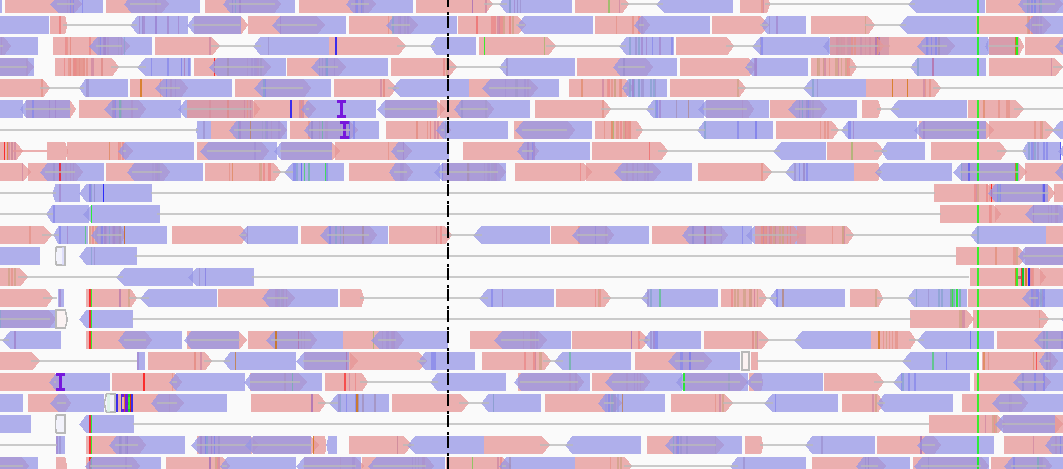
\includegraphics[width=0.6\textwidth]{pos1.PNG}
\end{figure}

\begin{figure}[H]
    \caption{\textbf{\textit{chr5:9,410,315-9,413,699}}: it is quite clear that both the alleles were deleted in that region, because of the decrease in coverage}
    \centering
    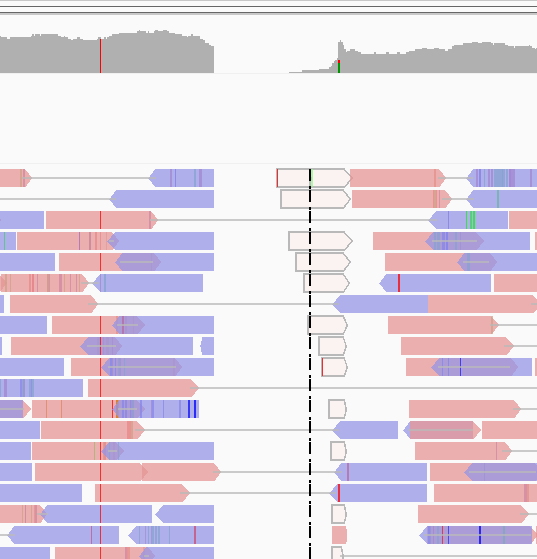
\includegraphics[width=0.55\textwidth]{pos2.PNG}
\end{figure}

\begin{figure}[H]
    \centering
    
    \begin{subfigure}[t]{0.55\textwidth}
        \centering
        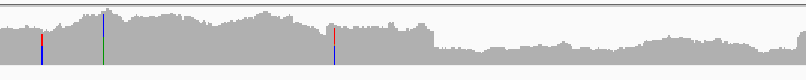
\includegraphics[width=1\textwidth]{cov3.PNG}
    \end{subfigure}
    \begin{subfigure}[t]{0.55\textwidth}
        \centering
        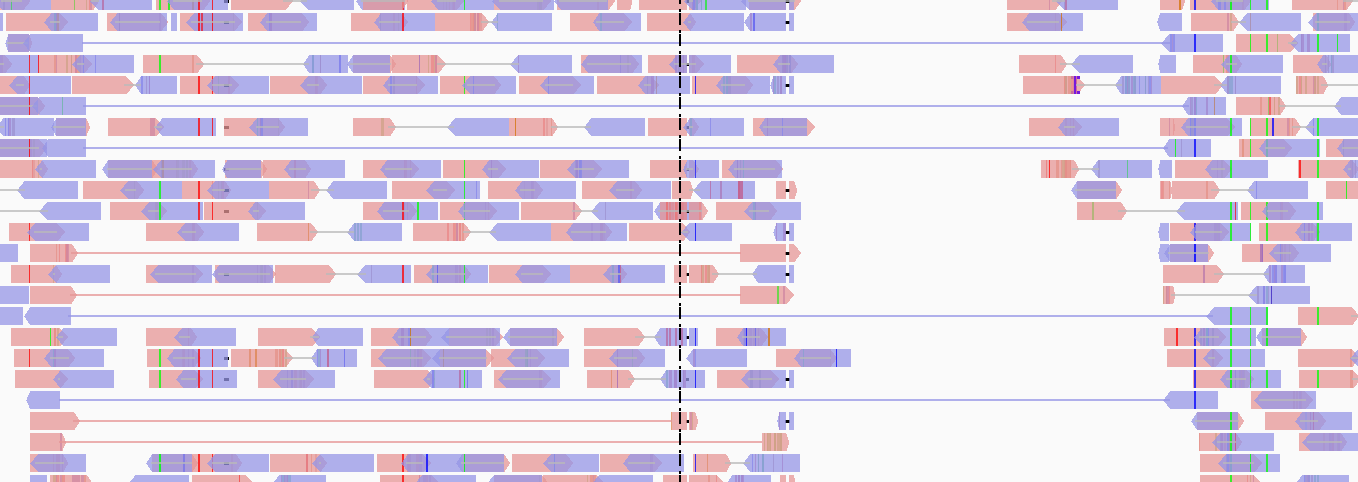
\includegraphics[width=1\textwidth]{pos3.PNG}
    \end{subfigure}
    \caption{\textit{\textbf{chr7:31,576,117-31,599,940}}: Basically you have an inversion between B and F, and after the deletion of the ED portion, the other allele remains normal.}
    \label{fig:3}
\end{figure}

%#TODO complete all the figures of the exercise

